%%%%%%%%%%%%%%%%%%%%%%%%%%%%%%%%%%%%%%%%%%%%%%%%%%%%%%%%%%%%%%%%%%%%%%%%%%%%%%%%
\chapter{Expression Tree Language}

\section{Formal grammar specification}

\begin{lstlisting}[caption={BNF formal ETL grammar specification.},
                   label={lst:etl-grammar}]
<forest> ::= <forest> <node> 
<forest> ::= ""
<node> ::= "(" <nodeContents> ")" <optNodeType>
<nodeContents> ::= <nodeContents> <nodeContent>
<nodeContents> ::= ""
<nodeContent> ::= <node>
<nodeContent> ::= "()"
<nodeContent> ::= <string>
<nodeContent> ::= "d" <string>
<nodeContent> ::= "u" <string>
<nodeContent> ::= <regex>
<nodeContent> ::= "_"
<nodeContent> ::= <nodeContent> "|" <nodeContent>
<nodeContent> ::= <nodeContent> "?"
<nodeContent> ::= <nodeContent> "+"
<nodeContent> ::= <nodeContent> "*"
<nodeContent> ::= "[" <nodeContent> <nodeContents> "]"
<optNodeType> ::= nodeType
<optNodeType> ::= ""
<nodeType> ::= ":" <TYPE_CHARS>
<string> ::= "\"" <STRING_CHARS> "\""
<regex>  ::= "/" <REGEX_CHARS> "/"
\end{lstlisting}

\section{Query matching algorithm}

\begin{lstlisting}[caption={Pseudo–code implementation of
                            the query–matching algorithm.},
                   label={lst:etl-query-algo},
                   language=pseudocode]
def match(query_node, target_node, query_root):
    type_match_if_present = len(query_node.type) > 0 and
                            query_node.type == target_node.type
    contents_match = vm_match(query_node.contents, target_node.contents)
    if contents_match and type_match_if_present:
      # Match process completed
      return true
    else:
      # Visit children starting from the query root
      return target_node.contents
        .filter(\it -> it is Node)
        .any(\it -> match(query_root, it, query_root))

def vm_match(query, target):
    program = vm_compile(query)
    matched = vm_exec(program,
                      target,
                      \it pos -> vm_match_child(query, pos, it))
    return matched == len(target)

def vm_exec(program, input, match_child):
    # implement backtracking by using "threads"
    threads = Queue()
    threads.add(Thread(0, 0, Stack()))
    while len(threads) > 0:
        result = vm_run_thread(program, input, match_child,
                               threads.pop(), threads.add,
                               \() -> len(threads) > 0)
        if result >= 0:
            return result
        # else: backtrack
    return -1

def vm_run_thread(program, input, match_child,
                  t, spawn_thread, is_last_thread):
    prog_len = len(program)
    input_len = len(input)
    pc = t.pc
    ic = t.ic

    while pc < prog_len:
        instr = program[pc]
        if instr is Instr.Elem:
            # elem: match against the target element
            if ic < input_len and match_elem(instr, input[ic]):
                pc += 1
                ic += 1
            else:
                break
        else if instr is Instr.Jump:
            # jump: change PC
            pc = instr.dest
        else if instr is Instr.Child:
            if ic < input_len and match_child(input[ic], instr.pos):
                pc += 1
                ic += 1
            else:
                break
        else if instr is Instr.Mark:
            if (instr.value & 1) == 0:
                # Open group: save value to the stack
                t.groups.push(instr.value)
                pc += 1
            else:
                # Close group: expected value + 1 at the top
                # the stack
                if t.groups.pop() + 1 == instr.value:
                    pc += 1
                else:
                    break
        else if instr is Instr.Match:
            # Allow to return if
            # - All groups have been closed
            # - There are no pending threads and ic == input_len
            #   to avoid early returns (which would not yield a
            #   complete match regardless
            if len(t.groups) == 0 and
                   (ic == input_len or is_last_thread()):
               return ic
            else:
                break
    return -1
            
def vm_match_child(query, pos, target):
    if not(target is Hole or target is Node):
        return false

    query_element = query[pos]
    if query_elem is Node:
        # Assert types equality first, then match contents
        return target is Node and
               (len(query_elem.type) == 0 or
                query_elem.type == target.type) and
               vm_match(query_elem, target)
    else if query_elem is Hole:
        # Only check if the type matches if the target
        # is a node
        return target is Hole or
               len(query_elem.type) == 0 or
               query_elem.type == target.type
    else if query_elem is Group:
        # Recursively match a list of query nodes against
        # the target. This usually happens when there's
        # one non-optional element sorrounded by other
        # optional elements
        return vm_match(query_elem.contents, listOf(target))
    else:
        return false
\end{lstlisting}


\chapter{Automatic Activity Generation}

\section{GitHub Action workflow configuration}

\begin{lstlisting}[language=yaml,
                   caption={Example GitHub Workflow configuration.},
                   label={lst:impl-gi-workflow}]
name: Expression Tutor Activity
on:
  push:
    tags:
      - '*'
permissions:
  issues: write
  contents: read
jobs:
  et_activity_generation:
    runs-on: ubuntu-latest
    name: Activity generation
    steps:
      - name: Checkout
        uses: actions/checkout@v3
      - name: Expression Tutor Activity generation
        uses: LuCEresearchlab/expression-tutor-activity-generator@v1.0.0
        id: exps
        with:
          srcDir: 'src/main/java'
          count: 1
          activityGroup: 'my-activity-group'
          javaClassPath: 'libs'
          ghToken: ${{ secrets.GITHUB_TOKEN }}
\end{lstlisting}

\chapter{Expression Tutor APIs}

\begin{chapterBody}

\section{Activity Groups API}

An \texttt{ActivityGroup} instance is made of the following:
\begin{itemize}
    \item \texttt{uuid} $ \in $ String: An unique identifier for the Activity 
Group.
    \item \texttt{label} $ \in $ String: A label used to denote the Activity 
Group.
    \item \texttt{owner} $ \in $ String: The UUID of the Instructor that owns
this Activity Group.
    \item \texttt{query} $ \in $ Maybe<String>: An ETL query that can be used 
by the Automated Activity Generation to query for an expression used to create 
an Activity which will belong to this Group.
    \item \texttt{allowFeedback} $ \in $ Boolean: Whether activities that 
belong to this Group are allowed to display feedback to Students upon 
submission.
    \item \texttt{sharedReferenceSolution} $ \in $ Boolean: Whether all 
activities that belong to this Group are supposed to share the same Reference
Solution.
\end{itemize}

\noindent The Expression Tutor website provides the following API for operating 
on Activity Groups:

\begin{itemize}
    \item \texttt{GET /api/activities/group}
    \begin{itemize}
        \item Retrieve all the Activity Groups owned by the instructor 
associated  with the token provided in the Authorization header.
        \item Request:
        \begin{itemize}
            \item Headers: \texttt{Authorization}
        \end{itemize}
        \item Response: list of \texttt{ActivityGroup}s
    \end{itemize}
    \item \texttt{POST /api/activities/group}
    \begin{itemize}
        \item Create a new Activity Group owned by the instructor associated 
with the token provided in the Authorization header.
        \item Request:
        \begin{itemize}
            \item Headers: \texttt{Authorization}
            \item Body:
            \begin{itemize}
                \item \texttt{label} $ \in $ String: A label used to denote 
the Activity Group.
            \end{itemize}
        \end{itemize}
        \item Response: an \texttt{ActivityGroup}
    \end{itemize}
    \item \texttt{GET /api/activities/group/\{uuid\}}
    \begin{itemize}
        \item Update the contents of the Activity Group identified by the
UUID specified in the path.
        \item Request:
        \begin{itemize}
            \item Headers: \texttt{Authorization}
        \end{itemize}
        \item Response: an \texttt{ActivityGroup}
    \end{itemize}
    \item \texttt{PATCH /api/activities/group/\{uuid\}}
    \begin{itemize}
        \item Update the contents of the Activity Group identified by the
UUID specified in the path. This operation is allowed only if the Instructor
associated with the token provided in the Authorization header is the owner of
the Activity Group or has the ``Administrator role''.
        \item Request:
        \begin{itemize}
            \item Headers: \texttt{Authorization}
            \item Body:
            \begin{itemize}
                \item \texttt{label} $ \in $ Maybe<String>
                \item \texttt{query} $ \in $ Maybe<String>
                \item \texttt{allowFeedback} $ \in $ Maybe<Boolean>
                \item \texttt{sharedReferenceSolution} $ \in $ Maybe<Boolean>
            \end{itemize}
        \end{itemize}
        \item Response: the updated \texttt{ActivityGroup}
    \end{itemize}
    \item \texttt{DELETE /api/activities/group/\{uuid\}}
    \begin{itemize}
        \item Delete the contents of the Activity Group identified by the
UUID specified in the path. This operation is allowed only if the Instructor
associated with the token provided in the Authorization header is the owner of
the Activity Group or has the ``Administrator role''.
        \item Request:
        \begin{itemize}
            \item Headers: \texttt{Authorization}
        \end{itemize}
        \item Response: an \texttt{ActivityGroup}
    \end{itemize}
    \item \texttt{GET /api/activities/group/\{uuid\}/report}
    \begin{itemize}
        \item Obtain an assessment report for the Activities that belong to the
Activity Group identified by the UUID specified in the path.
        \item Request:
        \begin{itemize}
            \item Headers: \texttt{Authorization}
        \end{itemize}
        \item Response: an \texttt{AssessmentReport} (see
Section~\ref{sec:fb-assess}).
    \end{itemize}
\end{itemize}

\section{Assessment API}

An \texttt{Submission} instance is made of the following:
\begin{itemize}
    \item \texttt{uuid} $ \in $ String: the unique identifier of the
submission.
    \item \texttt{submission} $ \in $ ExpressionTreeDiagram: Expression
Tree Diagram JSON representation of the student's submission.
    \item \texttt{reference} $ \in $ ExpressionTreeDiagram: Expression
Tree Diagram JSON representation of the reference solution.
\end{itemize}

\begin{itemize}
    \item \texttt{GET /api/activities/assess/diagram/\{uuid\}}
    \begin{itemize}
        \item Obtain the Expression Tree Diagrams of the submission 
identified by the \texttt{uuid} in the path and its associated reference
solution.
        \item Request:
        \begin{itemize}
            \item Headers: \texttt{Authorization}
        \end{itemize}
        \item Response: a \texttt{Submission instance}
    \end{itemize}
    \item \texttt{POST /api/activities/assess/feedback/structural}
    \begin{itemize}
        \item Obtain (structural) feedback for the given \texttt{Submission}
instances. Used to generate Formative Feedback for Students
(Section~\ref{sec:fb-ff}).
        \item Request:
        \begin{itemize}
            \item Body: an array of \texttt{Submission} instances
(the \texttt{reference} value is optional and will be retrieved
internally if it's missing to allow non–instructors to use this
feature).
        \end{itemize}
        \item Response:
        \begin{itemize}
            \item \texttt{observed}, \texttt{violated}: array of:
            \begin{itemize}
                \item \texttt{type} $ \in $ String: category of the
property.
                \item \texttt{description} $ \in $ String: descriptor
of the property.
            \end{itemize}
        \end{itemize}
    \end{itemize}
    \item \texttt{POST /api/activities/assess/feedback/treeColoring}
    \begin{itemize}
        \item Color the given Expression Tree Diagram according to
tree coloring information produced by the Assessment System
(Section~\ref{sec:fb-assess-color}).
        \item Request: a \texttt{Submission} instance (the
\texttt{reference} value is optional and will be retrieved internally
if it's missing to allow non–instructors to use this feature).
        \item Response: an \texttt{ExprTreeDiagram} instance with each
construct augmented with coloring information.
    \end{itemize}
    \item \texttt{POST /api/activities/assess/reference/}
    \begin{itemize}
        \item Create a new reference solution.
        \item Request:
        \begin{itemize}
            \item Body: an \texttt{ExprTreeDiagram} instance.
        \end{itemize}
        \item Response:
        \begin{itemize}
            \item \texttt{success} $ \in $ Boolean
            \item \texttt{uuid} $ \in $ Maybe<String>: the uuid of the
newly created reference solution.
        \end{itemize}
    \end{itemize}
    \item \texttt{GET /api/activities/assess/reference/\{uuid\}}
    \begin{itemize}
        \item Retrieve the reference solution associated with the identifier
specified in the path.
        \item Request:
        \begin{itemize}
            \item Headers: \texttt{Authorization}
        \end{itemize}
        \item Response: an \texttt{ExprTreeDiagram} instance
    \end{itemize}
    \item \texttt{PATCH /api/activities/assess/reference/\{uuid\}}
    \begin{itemize}
        \item Update a reference solution.
        \item Request:
        \begin{itemize}
            \item Headers: \texttt{Authorization}
            \item Body: an \texttt{ExprTreeDiagram} instance.
        \end{itemize}
        \item Response: an \texttt{ExprTreeDiagram} instance.
    \end{itemize}
    \item \texttt{POST /api/activities/assess}
    \begin{itemize}
        \item Obtain an assessment for the given submissions.
        \item Request:
        \begin{itemize}
            \item Headers:
            \begin{itemize}
                \item \texttt{Authorization}
                \item \texttt{Accept}: one of \texttt{application/json}
(default) or \texttt{text/csv}
            \end{itemize}
            \item Body: an array of:
            \begin{itemize}
                \item \texttt{type} $ \in $ String. Type of the assessment
object to generate. One of \texttt{details}, \texttt{grading} or
\texttt{incorrectNodes}.
                \item \texttt{uuids} $ \in $ List<String>. List of uuids
of the submissions to generate an assessment for.
            \end{itemize}
        \end{itemize}
        \item Response: either a JSON or CSV document (depending on the
request) containing an assessment report (see Section~\ref{sec:fb-assess}).
    \end{itemize}
\end{itemize}

\section{Instructors API}

An \texttt{Instructor} instance is made of the following:
\begin{itemize}
    \item \texttt{uuid} $ \in $ String: An immutable unique identifier for the 
instructor.
    \item \texttt{label} $ \in $ String: A label used to denote the instructor.
    \item \texttt{token} $ \in $ String: The instructor's token.
    \item \texttt{role} $ \in $ String: The role assigned to the instructor.
\end{itemize}

\begin{itemize}
    \item \texttt{GET /api/instructor}
    \begin{itemize}
        \item Retrieve information about the instructor associated with the token
that has been provided in the \texttt{Authorization} header.
        \item Request:
        \begin{itemize}
            \item Headers: \texttt{Authorization}
        \end{itemize}
        \item Response: an \texttt{Instructor} instance,
    \end{itemize}
\item \texttt{POST /api/instructor}
    \begin{itemize}
        \item Create a new instructor. This newly created instructor has the
``Admin'' role if it's the first instructor ever created in the database,
otherwise it has the ``Unauthorized'' role.
        \item Request:
        \begin{itemize}
            \item Body:
            \begin{itemize}
                \item \texttt{label} $ \in $ String: the label of the newly 
created instructor.
            \end{itemize}
        \end{itemize}
        \item Response: the updated \texttt{Instructor} instance.
    \end{itemize}
    \item \texttt{PATCH /api/instructor}
    \begin{itemize}
        \item Update the instructor which token has been provided in the
\texttt{Authorization} header.
        \item Request:
        \begin{itemize}
            \item Headers: \texttt{Authorization}
            \item Body:
            \begin{itemize}
                \item \texttt{label} $ \in $ \texttt{Maybe<String>}:
the new label of the instructor.
                \item \texttt{newToken} $ \in $ \texttt{Maybe<Boolean>}:
whether a new token should be issued.
            \end{itemize}
        \end{itemize}
        \item Response: the updated \texttt{Instructor} instance.
    \end{itemize}
    \item \texttt{DELETE /api/instructor}
    \begin{itemize}
        \item Delete the instructor which token has been provided in the
\texttt{Authorization} header
        \item Request:
        \begin{itemize}
            \item Headers: \texttt{Authorization}
        \end{itemize}
        \item Response: whether the deletion was successful or not.
    \end{itemize}
    \item \texttt{GET /api/instructor/admin}
    \begin{itemize}
        \item If the instructor, which token has been provided in the
\texttt{Authorization} header, has the ``Administrator'' role,
provides a list of all existing instructors.
        \item Request:
        \begin{itemize}
            \item Headers: \texttt{Authorization}
        \end{itemize}
        \item Response: list of \texttt{Instructor}s.
    \end{itemize}
    \item \texttt{DELETE /api/instructor/admin}
    \begin{itemize}
        \item If the instructor, which token has been provided in the
\texttt{Authorization} header, has the ``Administrator'' role,  delete an
instructor.
        \item Request:
        \begin{itemize}
            \item Headers: \texttt{Authorization}
            \item Body:
            \begin{itemize}
                \item \texttt{uuid} $ \in $ \texttt{String}: UUID of the 
instructor to delete.
            \end{itemize}
        \end{itemize}
        \item Response: whether the deletion was successful or not.
    \end{itemize}
    \item \texttt{PATCH /api/instructor/admin/role}
    \begin{itemize}
        \item If the instructor, which token has been provided in the
\texttt{Authorization} header, has the ``Administrator'' role,  update the role
of an instructor.
        \item Request:
        \begin{itemize}
            \item Headers: \texttt{Authorization}
            \item Body:
            \begin{itemize}
                \item \texttt{uuid} $ \in $ \texttt{String}:
UUID of the instructor which role should be updated.
                \item \texttt{role} $ \in $ \texttt{String}: the role to assign
to the \textit{target} instructor.
            \end{itemize}
        \end{itemize}
        \item Response: the updated \texttt{Instructor} instance.
    \end{itemize}
    \item \texttt{PATCH /api/instructor/admin/token}
    \begin{itemize}
        \item If the instructor, which token has been provided in the
\texttt{Authorization} header, has the ``Administrator'' role, invalidate an
issue a new token for an instructor.
        \item Request:
        \begin{itemize}
            \item Headers: \texttt{Authorization}
            \item Body:
            \begin{itemize}
                \item \texttt{uuid} $ \in $ \texttt{String}: UUID of the
\textit{target} instructor.
            \end{itemize}
        \end{itemize}
        \item Response: the updated \texttt{Instructor} instance.
    \end{itemize}
\end{itemize}

\chapter{Expression Service}

\begin{landscape}
\begin{figure}[ht]
    \centering
    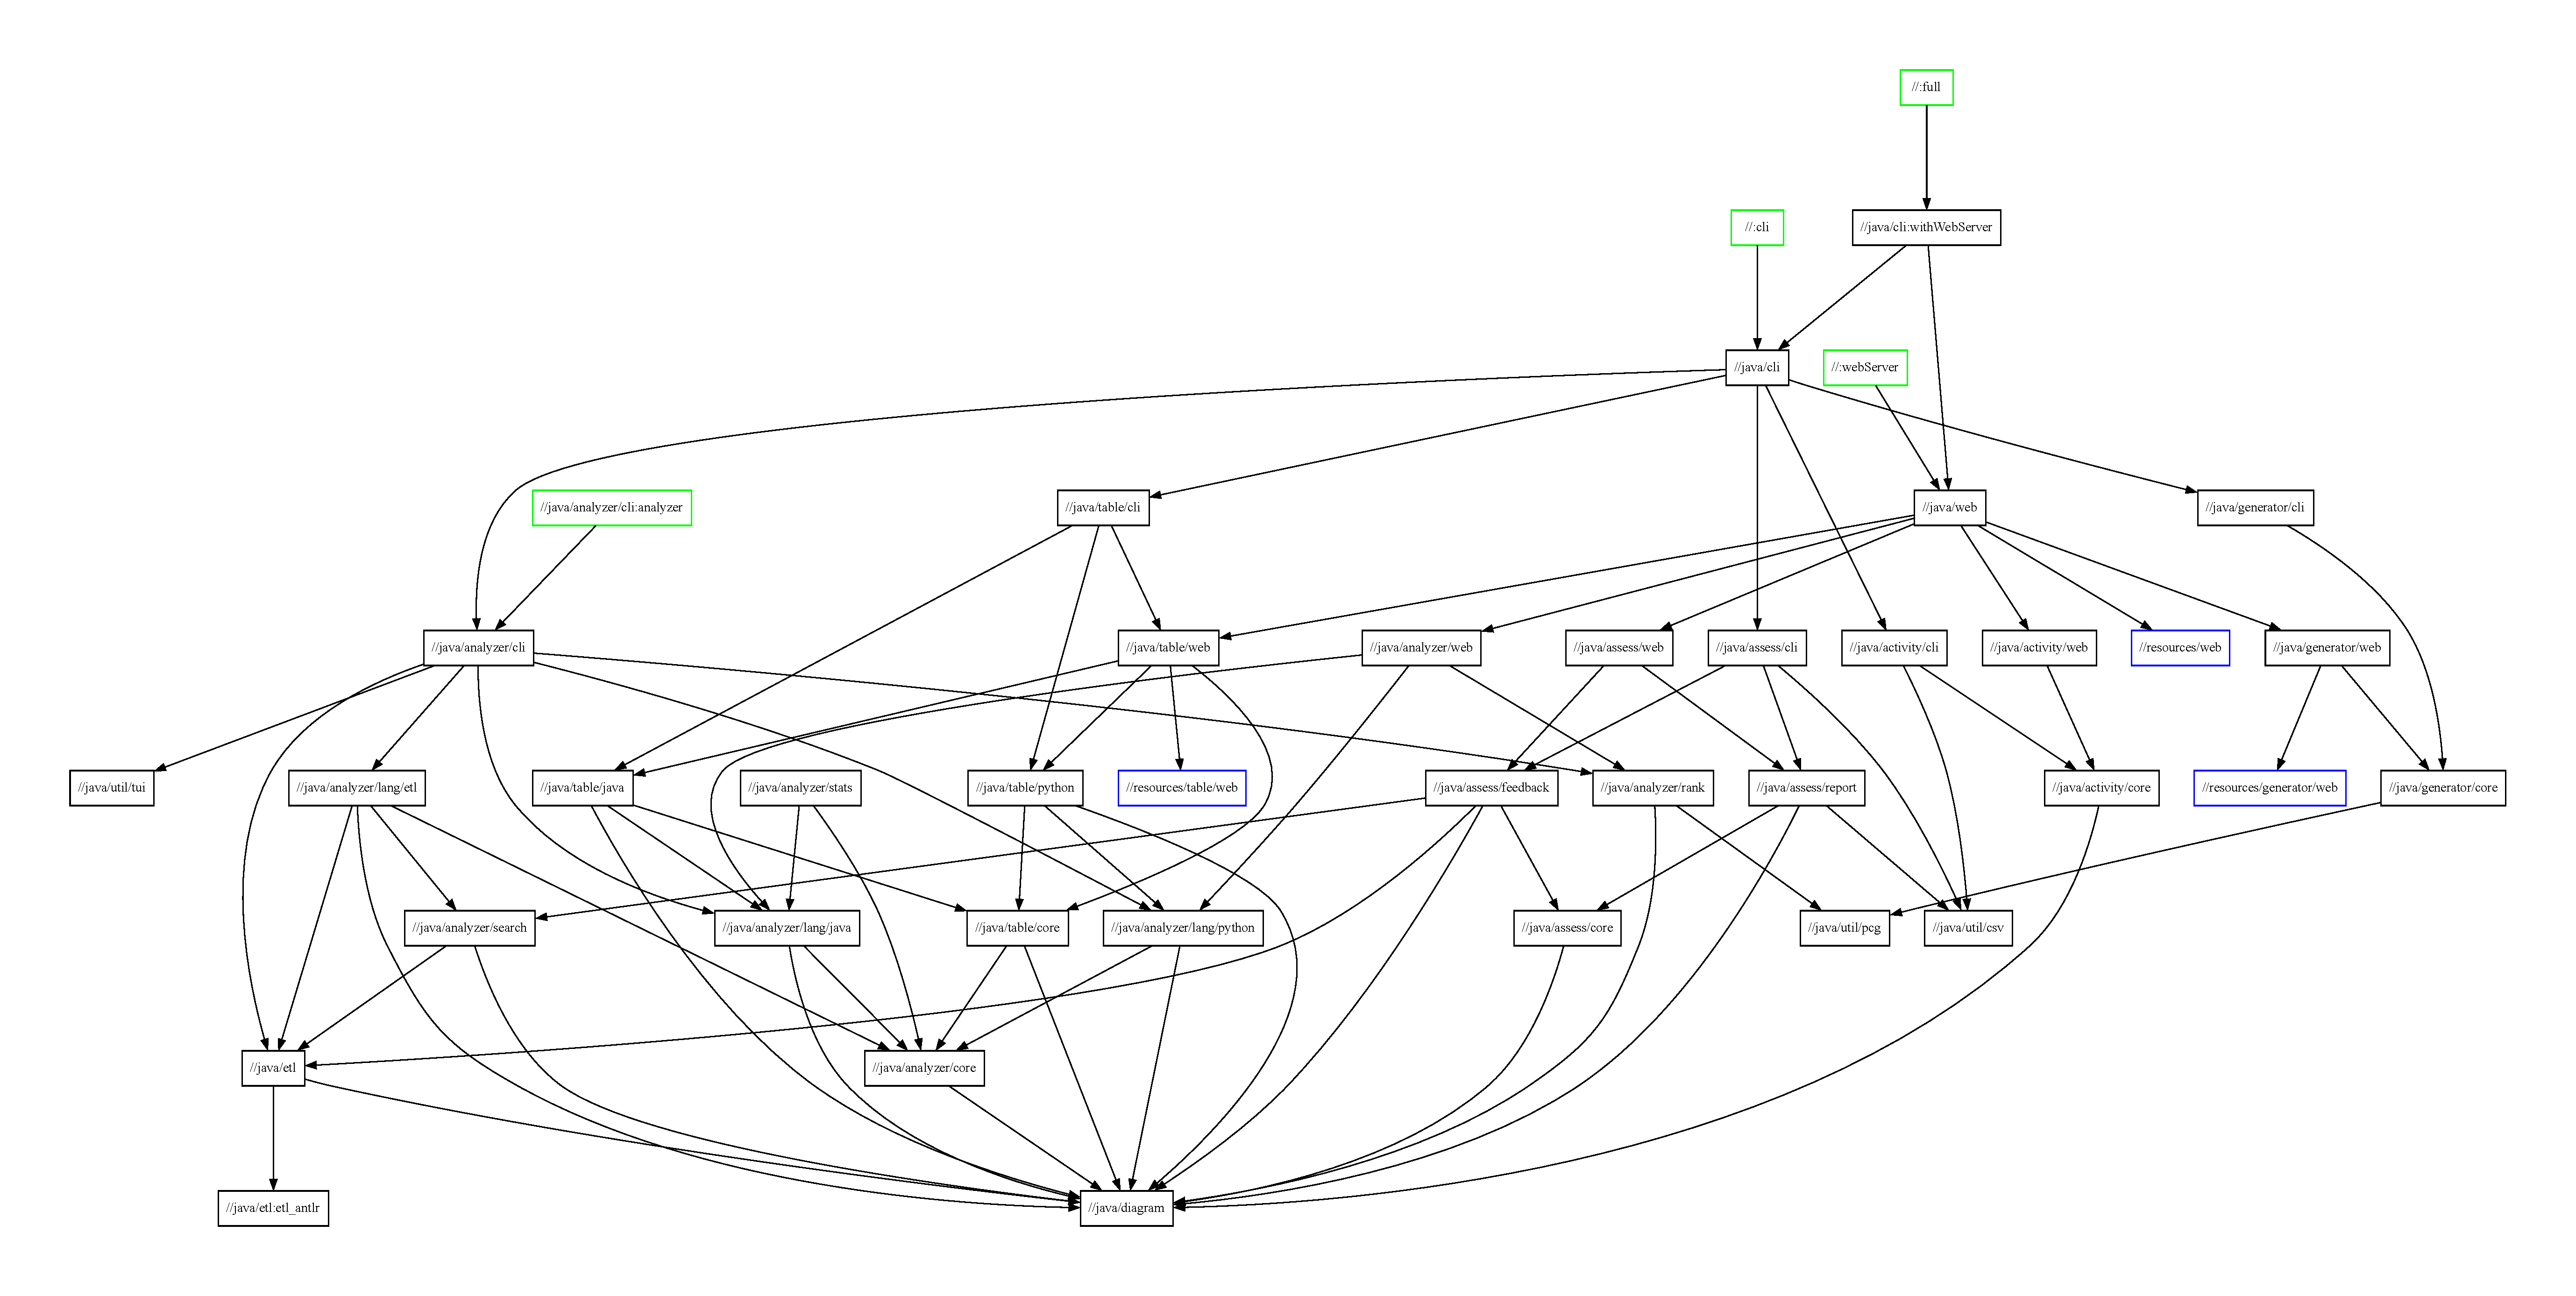
\includegraphics[width=\linewidth]{res/2/expr_serv_dep_graph.pdf}
    \caption{Architecture of Expression Service.}
    \label{fig:bg-es-arch}
\end{figure}
\end{landscape}

\end{chapterBody}